\section{Überblick}
\begin{frame}
	\frametitle{Übersicht Clock Pendulum Analyzer}
	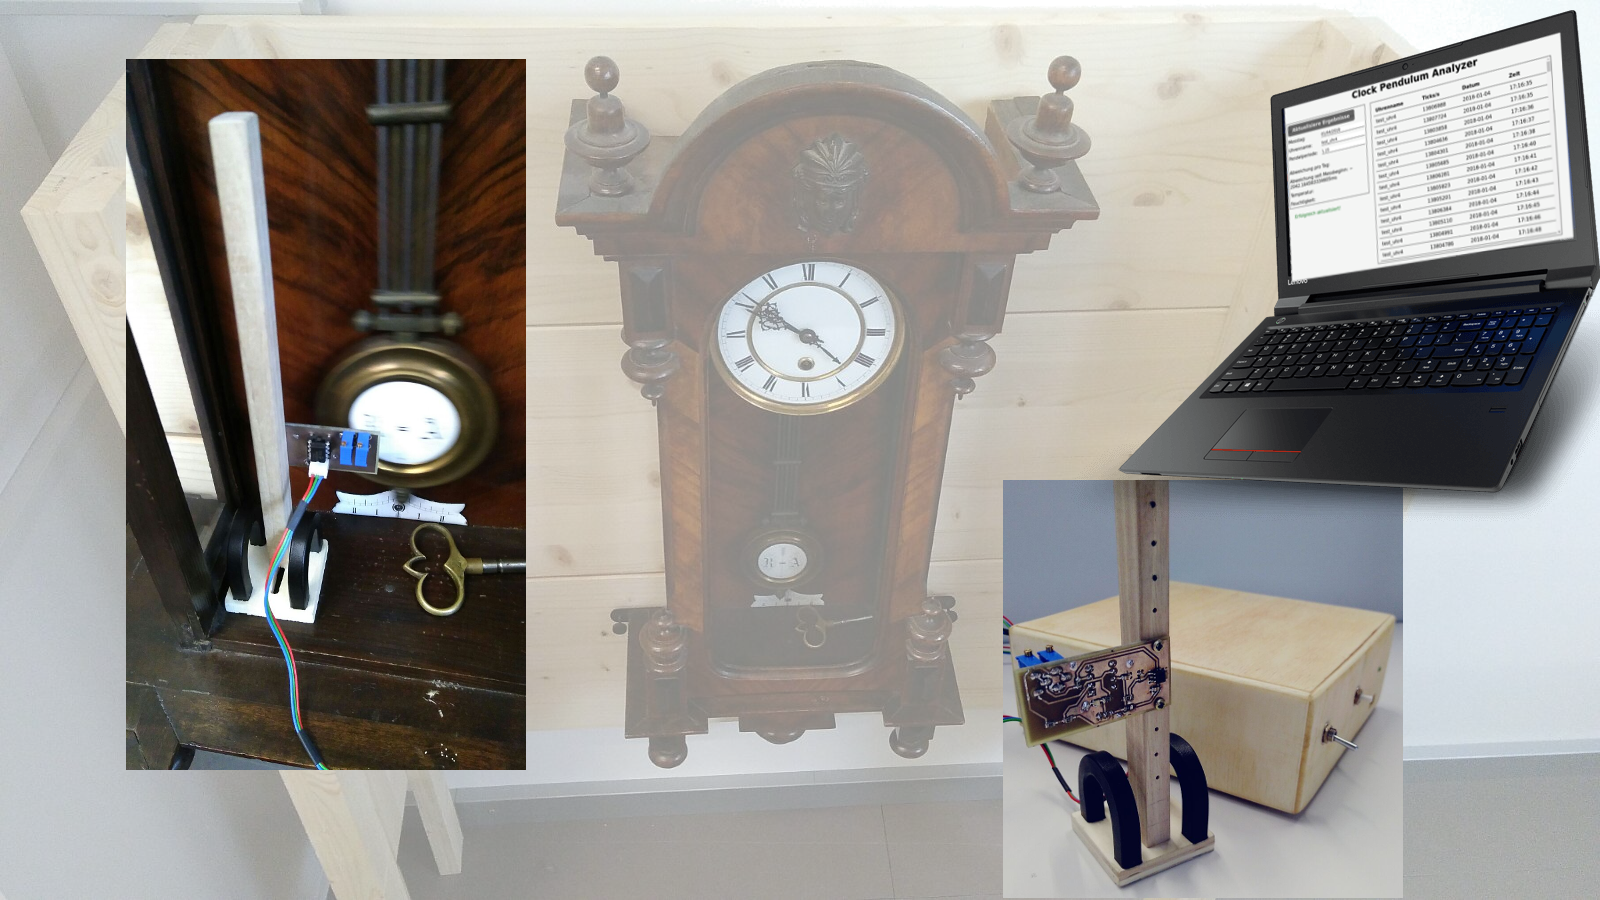
\includegraphics[width=\textwidth]{overview_system_title}
\end{frame}

\subsection{Funktionsumfang}
\begin{frame}
	\frametitle{Funktionsumfang}
	\begin{itemize}
		\item Messung verschiedener Pendeltypen im Mikrosekundenbereich.
		\item GPS-Disziplinierte Referenzfrequenz zur Ermittlung der vergangenen Zeit.
		\item Web- UI zur Darstellung der Messwerte.
		\item Unterschiedliche Pendel Periodendauern unterstützt.
		\item Schalter zur Unterscheidung, ob das Pendel den Sensor ganz passiert oder nicht.
		\item Bedienung direkt am Gerät und via Web- UI.
	\end{itemize}
\end{frame}